% Asset ID: A22ProjectilesTikZ-002
% Purpose: Show horizontal and vertical motion as separate component models.
\documentclass[tikz,border=8pt]{standalone}
\usepackage{amsmath}
\usetikzlibrary{arrows.meta,positioning}
\begin{document}
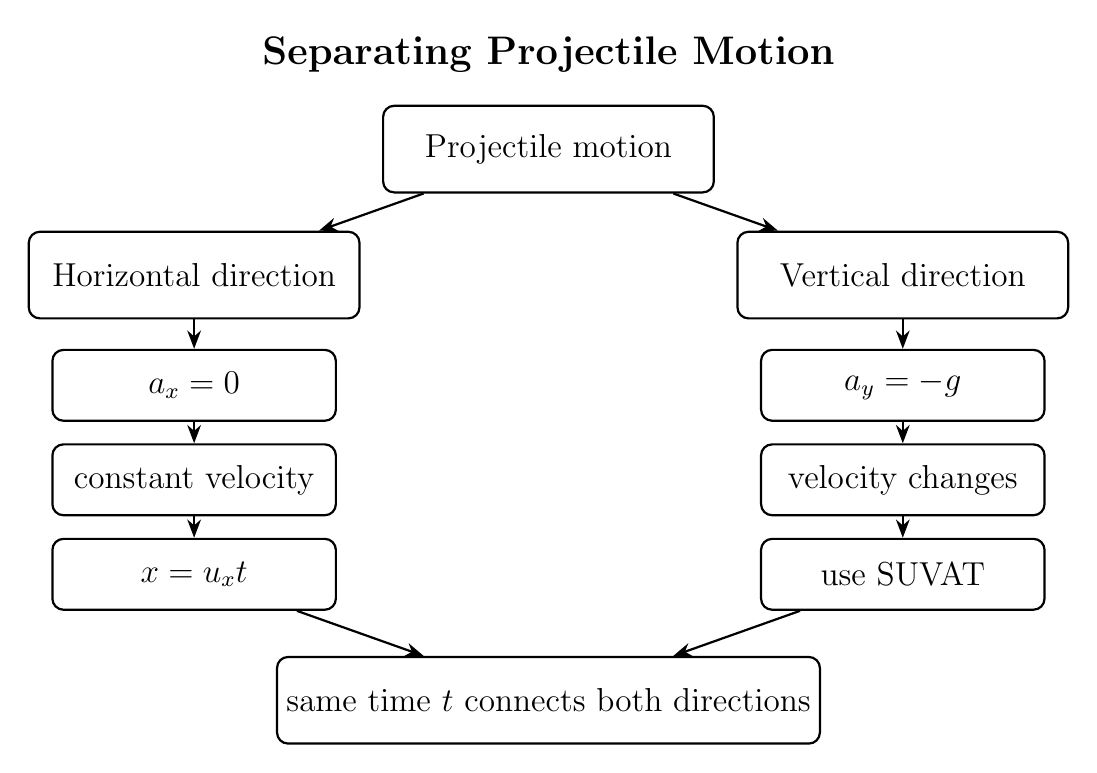
\begin{tikzpicture}[>=Stealth,box/.style={draw,rounded corners,thick,align=center,minimum width=4.2cm,minimum height=1.1cm,font=\large},smallbox/.style={draw,rounded corners,thick,align=center,minimum width=3.6cm,minimum height=0.9cm,font=\large},arrow/.style={->,thick},title/.style={font=\Large\bfseries}]
\node[title] at (0,4.2) {Separating Projectile Motion};
\node[box] (start) at (0,3) {Projectile motion}; \node[box] (horiz) at (-4.5,1.4) {Horizontal direction}; \node[box] (vert) at (4.5,1.4) {Vertical direction};
\draw[arrow] (start)--(horiz); \draw[arrow] (start)--(vert);
\node[smallbox] (hx0) at (-4.5,0) {$a_x=0$}; \node[smallbox] (hconst) at (-4.5,-1.2) {constant velocity}; \node[smallbox] (heqn) at (-4.5,-2.4) {$x=u_xt$};
\draw[arrow] (horiz)--(hx0); \draw[arrow] (hx0)--(hconst); \draw[arrow] (hconst)--(heqn);
\node[smallbox] (ay) at (4.5,0) {$a_y=-g$}; \node[smallbox] (vchange) at (4.5,-1.2) {velocity changes}; \node[smallbox] (suvat) at (4.5,-2.4) {use SUVAT};
\draw[arrow] (vert)--(ay); \draw[arrow] (ay)--(vchange); \draw[arrow] (vchange)--(suvat);
\node[box,minimum width=5.5cm] (time) at (0,-4.0) {same time $t$ connects both directions};
\draw[arrow] (heqn)--(time); \draw[arrow] (suvat)--(time);
\end{tikzpicture}
\end{document}
